\documentclass[final,hyperref={pdfpagelabels=false}]{beamer}
\usepackage{grffile}
\mode<presentation>{\usetheme{ECOMP}}
\usepackage[english]{babel}   
\usepackage[utf8]{inputenc}
\usepackage{amsmath,amsthm, amssymb, latexsym}
%\usepackage{times}\usefonttheme{professionalfonts}  % obsolete
%\usefonttheme[onlymath]{serif}
\boldmath
\usepackage[orientation=portrait,size=a0,scale=1.4,debug]{beamerposter}
% change list indention level
% \setdefaultleftmargin{3em}{}{}{}{}{}


%\usepackage{snapshot} % will write a .dep file with all dependencies, allows for easy bundling
\usepackage{csquotes}
\usepackage{array,booktabs,tabularx}
\newcolumntype{Z}{>{\centering\arraybackslash}X} % centered tabularx columns
\newcommand{\pphantom}{\textcolor{ta3aluminium}} % phantom introduces a vertical space in p formatted table columns??!!


%%%%%%%%%%%%%%%%%%%%%%%%%%%%%%%%%%%%%%%%%%%%%%%%%%%%%%%%%%%%%%%%%
\title{\Huge Implementation and Security Respectively Performance Evaluation of a Cache Covert Channel Cloud Scheduler}
\author{\huge Luthfi Idris\\[0.2\baselineskip]
\Large Supervisor: Prof. Dr. Dirk Westhoff and M. Sc. Johann Betz}
%\author[supervisor]{Supervisor:Prof.Dr.Dirk Westhoff and Johann Betz.Msc}
\institute{University of Applied Sciences Offenburg}
%%%%%%%%%%%%%%%%%%%%%%%%%%%%%%%%%%%%%%%%%%%%%%%%%%%%%%%%%%%%%%%%%
\newlength{\columnheight}
\setlength{\columnheight}{105cm}
%%%%%%%%%%%%%%%%%%%%%%%%%%%%%%%%%%%%%%%%%%%%%%%%%%%%%%%%%%%%%%%%
\begin{document}%Inicia o documento
\begin{frame}
  \begin{columns}%Inicia as Colunas
    % ---------------------------------------------------------%
    % Configurar a primeira coluna
\begin{column}{.49\textwidth}
      \begin{beamercolorbox}[center,wd=\textwidth]{postercolumn}
        \begin{minipage}[T]{.95\textwidth} % tweaks the width, makes a new \textwidth
          \parbox[t][\columnheight]{\textwidth}{ % must be some better way to set the the height, width and textwidth simultaneously
            % Since all columns are the same length, it is all nice and tidy.  You have to get the height empirically
            % ---------------------------------------------------------%
            % fill each column with content
            
            %%RESUMO%%%%%%%%%%%%%%%%%
\begin{block}{\Large \color{ta2skyblue} Introduction}
\Large
In Virtualization, scheduler effects on many parts of a cloud infrastructure. So that, selecting the right scheduler can optimize speed or increase security. Local scheduler defines access to the given resources from VMs on single physical machine while global scheduler defines the target physical machine on which VM should be started or migrated. 
\\

C3 scheduler intention is to mitigate the threat of leakage of information via cache covert channels by preventing processes to access cache lines alternately\cite{c1}.

% A local scheduler determines access to the give resources from VMs on a single physical machine. 
% The global scheduler determines the target physical machine on which a VM instance should be started or migrated.  

% C^{3}-Scheduler aiming at mitigating the threat of a leakage of customers data via cache covert channels by preventing processes to access cache lines alternately.

\end{block}


\begin{block}{\Large \color{ta2skyblue} Attack scenario}

\begin{figure}\vspace{0.5cm}
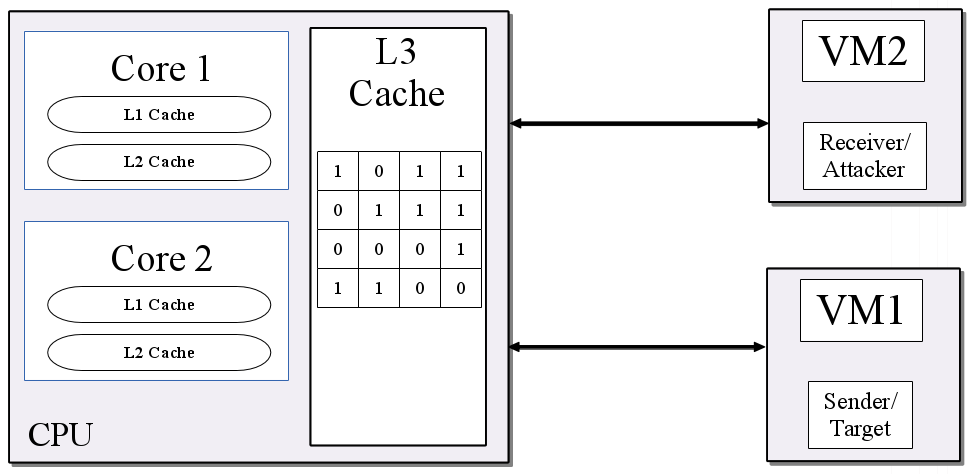
\includegraphics[width=0.8\linewidth]{cpu_cache.png}
\caption{\large CPU Cache Overview}
\end{figure}

\begin{figure}
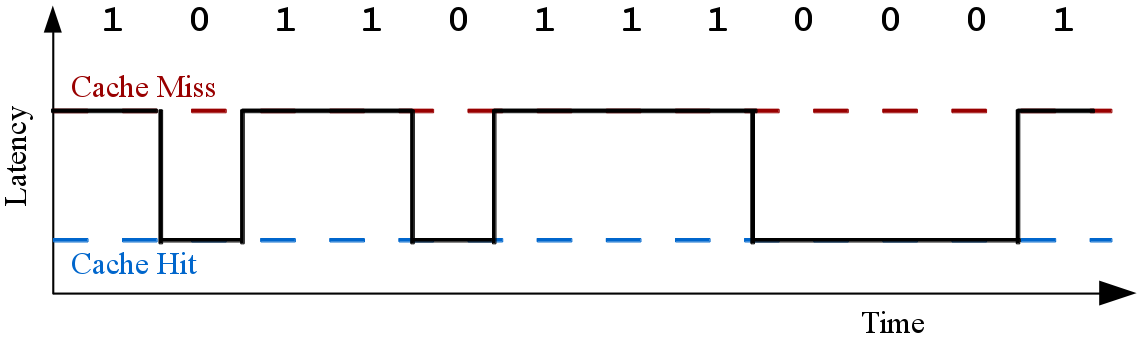
\includegraphics[width=0.9\linewidth]{time_patterns.png}
\caption{\large Timing Modulation Pattern \cite{c3}}
\end{figure}
\end{block}



%%%%%%%%%% Design and Implementation %%%%%%%%%%%%%
            
\begin{block}{\Large \color{ta2skyblue} Architecture}

\begin{figure}\vspace{1cm}
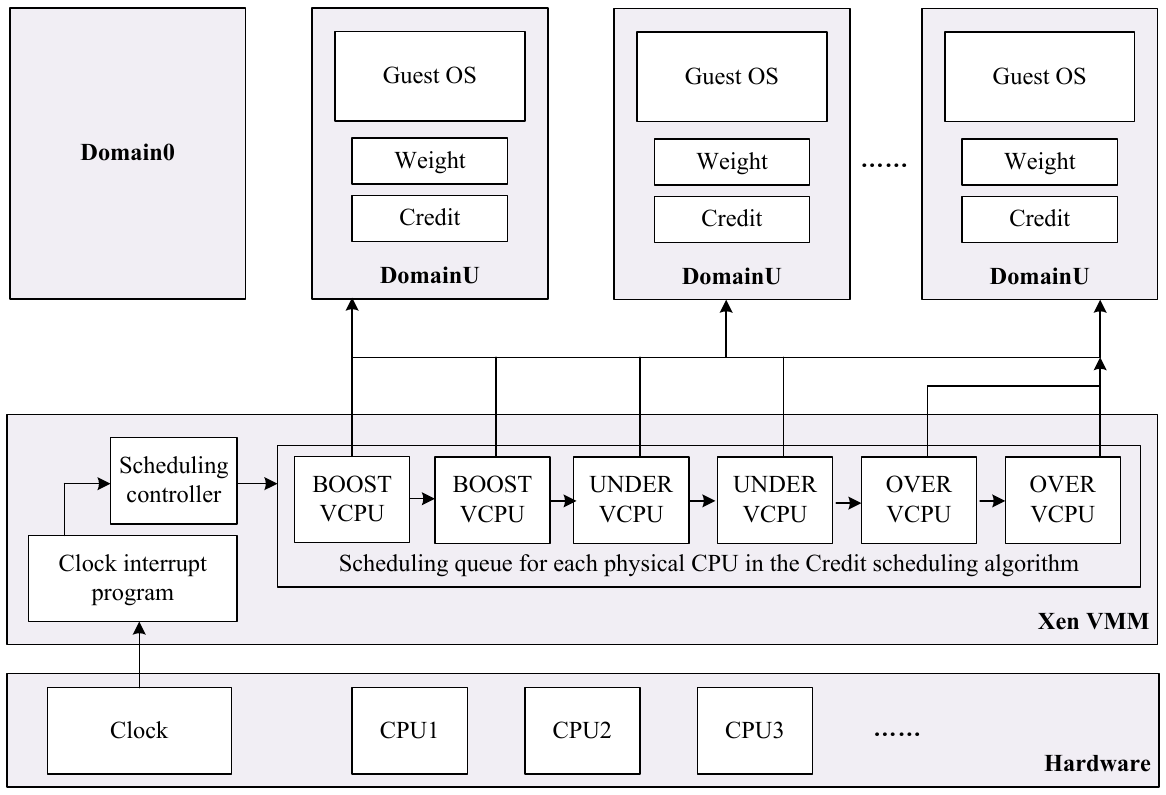
\includegraphics[width=1\linewidth]{credit_scheduler}
\caption{\large High Level Credit Scheduler\cite{c2}}
\end{figure}\vspace{1cm}


\end{block}
\vfill
        
          }
          % ---------------------------------------------------------%
          % end the column
        \end{minipage}
      \end{beamercolorbox}
    \end{column}
    % ---------------------------------------------------------%
    % Fim da coluna 1

    % ---------------------------------------------------------%
    % Ajuste da Coluna 2
\begin{column}{.49\textwidth}
\begin{beamercolorbox}[center,wd=\textwidth]{postercolumn}
\begin{minipage}[T]{.95\textwidth} % tweaks the width, makes a new \textwidth
\parbox[t][\columnheight]{\textwidth}{ 
         
           
%%%%%%%%%%OBJETIVOS%%%%%%%%%%%%%%
%\Large \color{black}

\begin{block}{\Large \color{ta2skyblue} Pseudo Code}

\begin{figure}
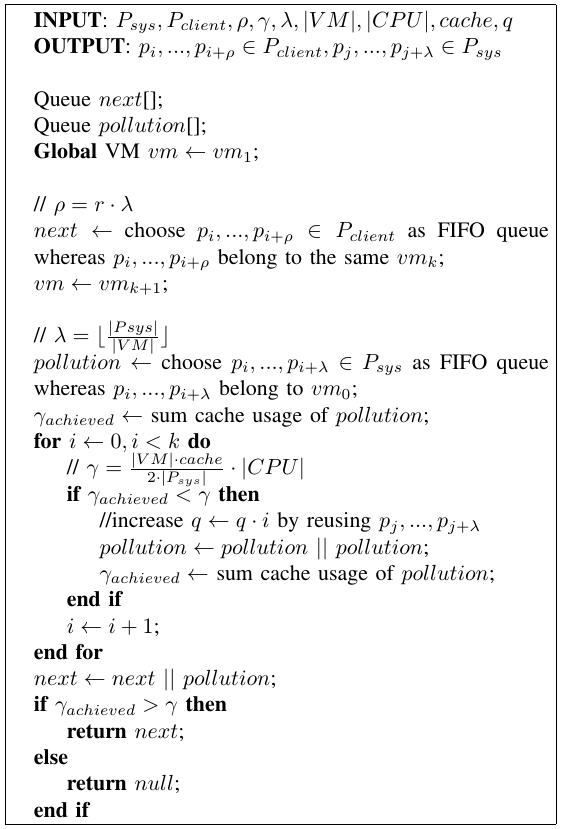
\includegraphics[width=0.55\linewidth]{pseudo_code.png}
\caption{\large Pseudo Code C3 Scheduler\cite{c1}}
\end{figure}
\end{block}

\begin{block}{\Large \color{ta2skyblue} Design Strategies and Objective}

\begin{figure}\vspace{1cm}
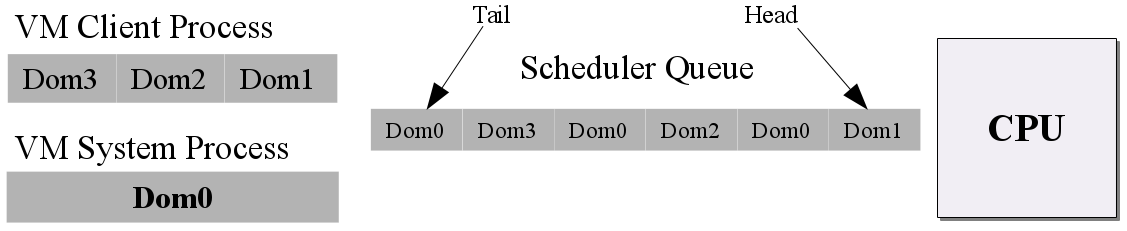
\includegraphics[width=0.9\linewidth]{c3_scheduler.png}
\caption{\color{black}\large C3 Scheduler}
\end{figure}

\begin{figure}\vspace{1cm}
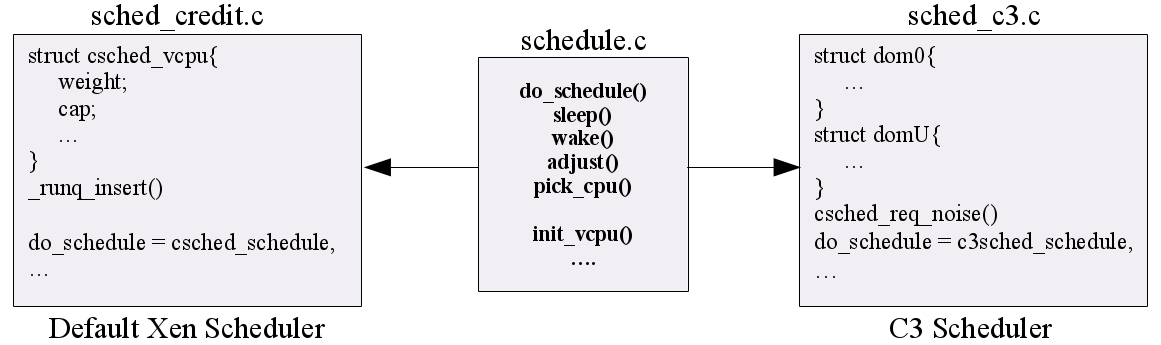
\includegraphics[width=0.85\linewidth]{c3_scheduler_framework.png}
\caption{\color{black}\large Xen Scheduler Framework}
\end{figure}\vspace{1cm}

\begin{itemize}
\item Implementing C3 Scheduler
\item Integrating to the Xen Hypervisor
\item Evaluating performance by simple program with and without using C3 Scheduler
\end{itemize}
 
\end{block}
%%%%%%%%%%%%%%%%%%%%%%%%%%%%%%%%%%%%%%%%%%%%%%%%%
           
%%%%%%%%%%%%%METODOLOGIA%%%%%%%%
\begin{block}{\Large \color{ta2skyblue} Reference}

\begin{thebibliography}{99}
\large
\bibitem{c1}\normalsize  Betz, Johann and Westhoff, Dirk: C3-Sched - A Cache Covert Channel robust Cloud Computing Scheduler, ICITST, pp. 55-61, Technical Co-Sponsored by IEEE UK/RI Computer Chapter, London, U.K., 2014.  
\bibitem{c2}\normalsize Zeng, L., Wang, Y., Shi, W., and Feng, D. An improved xen credit scheduler for i/o latency-sensitive applications on multicores. In Cloud Computing and Big Data (CloudCom-Asia), 2013 International Conference on (Dec 2013), pp. 267-274.
\bibitem{c3} \normalsize Wu, Zhenyu, Zhang Xu, and Haining Wang: Whispers in the hyper-space: High-speed covert channel attacks in the cloud. In Proceedings of the 21st USENIX Conference on Security Symposium, Security’12, pages 9–9, Berkeley, CA, USA, 2012. USENIX Association. http://dl.acm.org/citation.cfm?id=2362793.2362802.


\end{thebibliography}
\end{block}
\vfill          
\vfill


\begin{center}
\begin{tabular}{ccc}

\end{tabular}
\end{center}


          }
           
          % ---------------------------------------------------------%
          % end the column
        \end{minipage}
      \end{beamercolorbox}
    \end{column}
    % ---------------------------------------------------------%
    % end the column
  \end{columns}
  \vskip1ex
\end{frame}
\end{document}


%%%%%%%%%%%%%%%%%%%%%%%%%%%%%%%%%%%%%%%%%%%%%%%%%%%%%%%%%%%%%%%%%%%%%%%%